\documentclass[8pt,aspectratio=169]{beamer}
\usetheme{Madrid}
\usepackage{graphicx}
\usepackage{tikz}
\usepackage{pgfplots}
\pgfplotsset{compat=1.17}

% Define colors
\definecolor{maincolor}{RGB}{64,64,64}
\definecolor{lightgray}{RGB}{240,240,240}
\definecolor{midgray}{RGB}{180,180,180}
\definecolor{accentblue}{RGB}{70,130,180}

% Set theme colors
\setbeamercolor{structure}{fg=maincolor}
\setbeamercolor{title}{fg=maincolor}
\setbeamercolor{frametitle}{fg=maincolor,bg=lightgray}
\setbeamercolor{normal text}{fg=maincolor}
\setbeamercolor{item}{fg=maincolor}
\setbeamercolor{section in toc}{fg=maincolor}
\setbeamercolor{footline}{fg=midgray}

% Remove navigation symbols
\setbeamertemplate{navigation symbols}{}

% Custom footline
\setbeamertemplate{footline}{
    \leavevmode%
    \hbox{%
    \begin{beamercolorbox}[wd=.5\paperwidth,ht=2.5ex,dp=1ex,left]{author in head/foot}%
        \usebeamerfont{author in head/foot}\hspace{1em}\insertshortauthor
    \end{beamercolorbox}%
    \begin{beamercolorbox}[wd=.5\paperwidth,ht=2.5ex,dp=1ex,right]{date in head/foot}%
        \usebeamerfont{date in head/foot}\insertshortdate\hspace{1em}
        \insertframenumber{} / \inserttotalframenumber\hspace{1em}
    \end{beamercolorbox}}%
    \vskip0pt%
}

\title{\textbf{AI for Digital Finance}\\
\large Launching a Swiss-MENA Research Network}
\subtitle{Connect \& Collaborate Grant Application\\
Leading House MENA 2025}
\author{Prof. Joerg Osterrieder (FHGR) \& Prof. Stephen Chan (AUS)}
\date{April 21-23, 2026}

\begin{document}

\frame{\titlepage}

\begin{frame}{Agenda}
\tableofcontents
\end{frame}

\section{Project Overview}

\begin{frame}{Strategic Vision}
\begin{columns}
\begin{column}{0.48\textwidth}
\textbf{Mission}
\begin{itemize}
    \item Launch sustainable Swiss-MENA AI Finance Research Network
    \item Bridge academic research and industry practice
    \item Foster knowledge exchange between complementary ecosystems
\end{itemize}

\vspace{\fill}

\footnotesize\color{midgray}
Building on 7-year collaboration, 4 publications
\end{column}

\begin{column}{0.48\textwidth}
\textbf{Key Differentiators}
\begin{itemize}
    \item Swiss precision meets MENA market dynamics
    \item Both regions: global financial centers
    \item Complementary regulatory approaches
    \item Strong industry engagement (40\%)
\end{itemize}

\vspace{\fill}

\footnotesize\color{midgray}
80-100 participants expected
\end{column}
\end{columns}
\end{frame}

\begin{frame}{Workshop Focus Areas}
\begin{columns}
\begin{column}{0.48\textwidth}
\textbf{AI/ML Technologies}
\begin{itemize}
    \item Large Language Models (LLMs) in Finance
    \item Explainable AI for Compliance
    \item ML for Fraud Detection
    \item Predictive Analytics
\end{itemize}

\vspace{\fill}

\footnotesize\color{midgray}
Interdisciplinary: CS/AI, Finance, Mathematics
\end{column}

\begin{column}{0.48\textwidth}
\textbf{Application Domains}
\begin{itemize}
    \item Digital Banking Innovation
    \item Capital Markets \& Trading
    \item Risk Management
    \item Financial Inclusion
\end{itemize}

\vspace{\fill}

\footnotesize\color{midgray}
Focus on practical implementation
\end{column}
\end{columns}
\end{frame}

\section{Partnership Strength}

\begin{frame}{Proven Collaboration Track Record}
\begin{columns}
\begin{column}{0.48\textwidth}
\textbf{Research Achievements}
\begin{itemize}
    \item Extended research collaboration over 7 years at AUS
    \item 4 published papers:
    \begin{itemize}
        \footnotesize
        \item Blockchain security guide
        \item Advanced fraud detection methods
        \item NFTs in the Metaverse (2 papers)
    \end{itemize}
    \item Multiple grants secured
\end{itemize}

\vspace{\fill}

\footnotesize\color{midgray}
Established research foundation
\end{column}

\begin{column}{0.48\textwidth}
\textbf{International Network}
\begin{itemize}
    \item Dr. Yuanyuan Zhang (Manchester, UK)
    \item Prof. Jeffrey Chu (Renmin, China)
    \item Prof. Codruta Mare (Babes-Bolyai, Romania)
    \item Prof. Branka Hadji Misheva (Bern, Switzerland)
    \item MSCA Industrial Doctoral Network
\end{itemize}

\vspace{\fill}

\footnotesize\color{midgray}
Global perspectives and expertise
\end{column}
\end{columns}
\end{frame}

\section{Workshop Program}

\begin{frame}{Three-Day Structure}
\begin{columns}
\begin{column}{0.32\textwidth}
\textbf{Day 1: April 21}\\
\textit{Academic Foundations}
\begin{itemize}
    \footnotesize
    \item Opening ceremony
    \item Keynote: LLMs in Finance
    \item Research presentations
    \item Blockchain security session
    \item Research priorities panel
    \item Welcome reception
\end{itemize}
\end{column}

\begin{column}{0.32\textwidth}
\textbf{Day 2: April 22}\\
\textit{Industry Applications}
\begin{itemize}
    \footnotesize
    \item Keynote: UAE Finance
    \item Explainable AI session
    \item Digital banking cases
    \item Industry roundtable
    \item DIFC/ADGM participation
    \item Bank case studies
\end{itemize}
\end{column}

\begin{column}{0.32\textwidth}
\textbf{Day 3: April 23}\\
\textit{Network Launch}
\begin{itemize}
    \footnotesize
    \item MSCA doctoral training
    \item PhD presentations
    \item Working groups formation
    \item 5-year roadmap
    \item MoU signing
    \item Closing ceremony
\end{itemize}
\end{column}
\end{columns}

\vspace{\fill}

\footnotesize\color{midgray}
Location: American University of Sharjah, UAE
\end{frame}

\section{Budget and Funding}

\begin{frame}{Budget Overview - CHF 24,500 Total}

\begin{columns}
\begin{column}{0.48\textwidth}
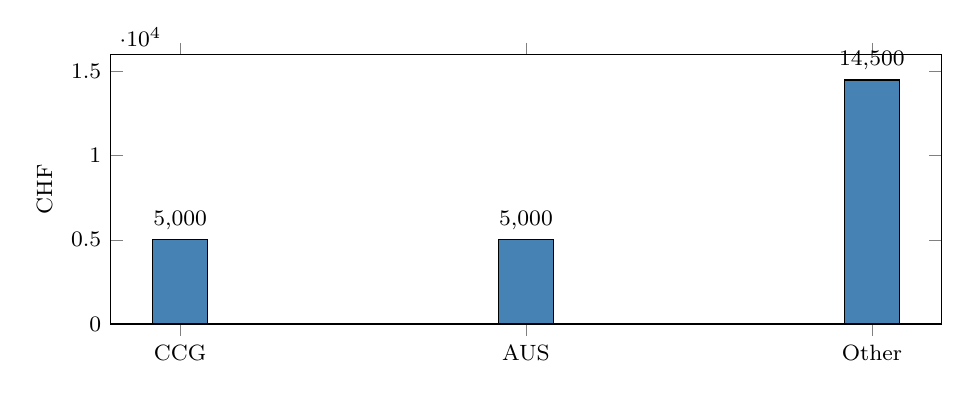
\begin{tikzpicture}
\begin{axis}[
    width=\textwidth,
    height=5cm,
    ybar,
    bar width=0.7cm,
    ylabel={CHF},
    symbolic x coords={CCG, AUS, Other},
    xtick=data,
    nodes near coords,
    nodes near coords align={vertical},
    ymin=0,
    ymax=16000,
    ylabel style={font=\footnotesize},
    xlabel style={font=\footnotesize},
    tick label style={font=\footnotesize},
    every node near coord/.append style={font=\footnotesize}
]
\addplot[fill=accentblue] coordinates {
    (CCG, 5000)
    (AUS, 5000)
    (Other, 14500)
};
\end{axis}
\end{tikzpicture}

\vspace{\fill}

\footnotesize\color{midgray}
CCG: 20.4\%, AUS: 20.4\%, Other: 59.2\%
\end{column}

\begin{column}{0.48\textwidth}
\textbf{CCG Request: CHF 5,000}
\begin{itemize}
    \item Travel: CHF 1,500
    \item Subsistence: CHF 800
    \item Catering: CHF 1,200
    \item Materials: CHF 300
    \item Platform: CHF 600
    \item Work costs: CHF 600 (12\%)
\end{itemize}

\textbf{Co-funding Sources}
\begin{itemize}
    \item AUS: CHF 5,000 (venue, equipment)
    \item Registration fees: CHF 8,000
    \item FHGR/sponsors: CHF 6,500
\end{itemize}

\vspace{\fill}

\footnotesize\color{midgray}
Work costs under 20\% limit
\end{column}
\end{columns}
\end{frame}

\section{Expected Impact}

\begin{frame}{Deliverables and Outcomes}
\begin{columns}
\begin{column}{0.48\textwidth}
\textbf{Tangible Outputs}
\begin{itemize}
    \item Workshop proceedings (open access)
    \item White paper on AI in Finance
    \item 5-year research agenda
    \item Online resource repository
    \item Video recordings and materials
\end{itemize}

\vspace{\fill}

\footnotesize\color{midgray}
All materials openly accessible
\end{column}

\begin{column}{0.48\textwidth}
\textbf{Strategic Impact}
\begin{itemize}
    \item Research network establishment
    \item Industry partnerships
    \item Publication pipeline
    \item Foundation for bilateral funding
    \item Policy influence (FINMA, UAE regulators)
\end{itemize}

\vspace{\fill}

\footnotesize\color{midgray}
Sustainable collaboration framework
\end{column}
\end{columns}
\end{frame}

\begin{frame}{Timeline and Next Steps}

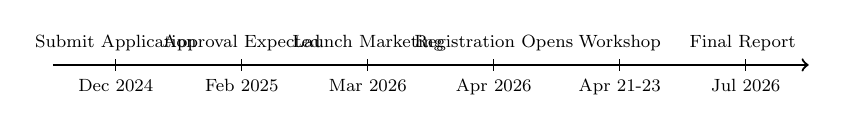
\begin{tikzpicture}[scale=0.8, transform shape]
\draw[thick, ->] (0,0) -- (12,0) node[anchor=north west] {};

% Timeline points
\foreach \x/\date/\event in {
    1/Dec 2024/Submit Application,
    3/Feb 2025/Approval Expected,
    5/Mar 2026/Launch Marketing,
    7/Apr 2026/Registration Opens,
    9/Apr 21-23/Workshop,
    11/Jul 2026/Final Report
} {
    \draw (\x,0) -- (\x,-0.1) node[below, align=center, font=\footnotesize] {\date};
    \draw (\x,0) -- (\x,0.1) node[above, align=center, font=\footnotesize] {\event};
}
\end{tikzpicture}

\vspace{1cm}

\textbf{Immediate Actions}
\begin{columns}
\begin{column}{0.48\textwidth}
\begin{itemize}
    \item Finalize application documents
    \item Secure AUS commitment letter
    \item Obtain industry support letters
    \item Submit by December 2024
\end{itemize}
\end{column}

\begin{column}{0.48\textwidth}
\begin{itemize}
    \item Confirm keynote speakers
    \item Establish organizing committee
    \item Create workshop website
    \item Begin partnership outreach
\end{itemize}
\end{column}
\end{columns}

\vspace{\fill}

\footnotesize\color{midgray}
Application deadline: 4 months before event
\end{frame}

\section{Conclusion}

\begin{frame}{Why This Application Will Succeed}
\begin{columns}
\begin{column}{0.48\textwidth}
\textbf{Strong Foundation}
\begin{itemize}
    \item Proven 7-year collaboration
    \item Published research outputs
    \item Established international network
    \item Track record of grant success
\end{itemize}

\vspace{\fill}

\footnotesize\color{midgray}
Built on solid partnership
\end{column}

\begin{column}{0.48\textwidth}
\textbf{Perfect CCG Alignment}
\begin{itemize}
    \item Clear MENA partnership (AUS)
    \item Mixed academic-industry audience
    \item Substantial co-funding (80\%)
    \item Strategic regional relevance
\end{itemize}

\vspace{\fill}

\footnotesize\color{midgray}
Meets all CCG criteria
\end{column}
\end{columns}

\vspace{1cm}

\begin{center}
\Large\textbf{Ready to Launch Swiss-MENA AI Finance Network}
\end{center}
\end{frame}

\begin{frame}{}
\begin{center}
\Large\textbf{Thank You}\\
\vspace{1cm}
\normalsize
Questions and Discussion\\
\vspace{2cm}
\footnotesize
Contact: lhmena@hes-so.ch\\
Prof. Joerg Osterrieder: joerg.osterrieder@fhgr.ch\\
Prof. Stephen Chan: schan@aus.edu
\end{center}
\end{frame}

\end{document}